% pitch_presentation.tex
% Customer Segmentation for an Italian Fashion Retailer
% Final Pitch Presentation — LUISS Data Science in Action 2025/26
%
% Compile: pdflatex pitch_presentation.tex  (run twice for page numbers)
%          or: latexmk -pdf pitch_presentation.tex

\documentclass[aspectratio=169,10pt]{beamer}

% ── Theme ─────────────────────────────────────────────────────────────────────
\usetheme{default}
\usefonttheme{structurebold}
\usepackage[T1]{fontenc}
\usepackage[utf8]{inputenc}
\usepackage{booktabs}
\usepackage{graphicx}
\usepackage{amsmath}
\usepackage{eurosym}

% ── Colour scheme (matches technical_report.tex) ──────────────────────────────
\definecolor{navy}{HTML}{1a1a2e}
\definecolor{accent}{HTML}{4361ee}
\definecolor{green}{HTML}{2e7d32}

\setbeamercolor{title}{bg=navy, fg=white}
\setbeamercolor{subtitle}{fg=white}
\setbeamercolor{author}{fg=white}
\setbeamercolor{institute}{fg=white!85}
\setbeamercolor{date}{fg=white!85}
\setbeamercolor{frametitle}{bg=navy, fg=white}
\setbeamercolor{structure}{fg=accent}
\setbeamercolor{block title}{bg=accent!15, fg=navy}
\setbeamercolor{block body}{bg=accent!5, fg=black}
\setbeamercolor{alertblock title}{bg=green!20, fg=green!60!black}
\setbeamercolor{alertblock body}{bg=green!5, fg=black}
\setbeamertemplate{navigation symbols}{}
\setbeamertemplate{footline}{%
  \hfill\color{navy}\footnotesize\insertframenumber/\inserttotalframenumber%
  \hspace{6pt}\vspace{4pt}}

% ── Metadata ──────────────────────────────────────────────────────────────────
\title{Six Segments, One Strategy Overhaul}
\subtitle{Data-Driven Customer Segmentation for an Italian Fashion Retailer}
\author{%
  \textbf{$\langle$NOME 1$\rangle$} \quad \textbf{$\langle$NOME 2$\rangle$}\\[2pt]
  \textbf{$\langle$NOME 3$\rangle$} \quad \textbf{$\langle$NOME 4$\rangle$}%
}
\institute{LUISS Guido Carli $\cdot$ Data Science in Action A.Y.\ 2025/26\\
  in partnership with \textbf{Jakala S.p.A.}}
\date{May 2026}

% =============================================================================
\begin{document}

% --- 1. Title slide -----------------------------------------------------------
\begin{frame}[plain]
\titlepage
\end{frame}

% --- 2. Hook slide ------------------------------------------------------------
\begin{frame}{\euro12M Revenue. Zero Customer Differentiation.}
\begin{columns}[T]
  \begin{column}{0.55\textwidth}
    \begin{block}{The opportunity gap}
    \small
    The retailer sends the \textbf{same campaigns} to:\\[4pt]
    \begin{tabular}{@{}ll@{}}
      \textbullet\ A VIP buying 5$\times$/year at \euro2{,}000 & \\
      \textbullet\ A bargain hunter buying only on promo & \\
      \textbullet\ A customer who has not returned in 14 months & \\
    \end{tabular}\\[6pt]
    This is not a personalisation problem.\\
    It is a \textbf{resource allocation problem}.
    \end{block}
    \vspace{0.4em}
    \textbf{Our answer:} identify who your customers actually are,
    then invest accordingly.
  \end{column}
  \begin{column}{0.42\textwidth}
    \centering
    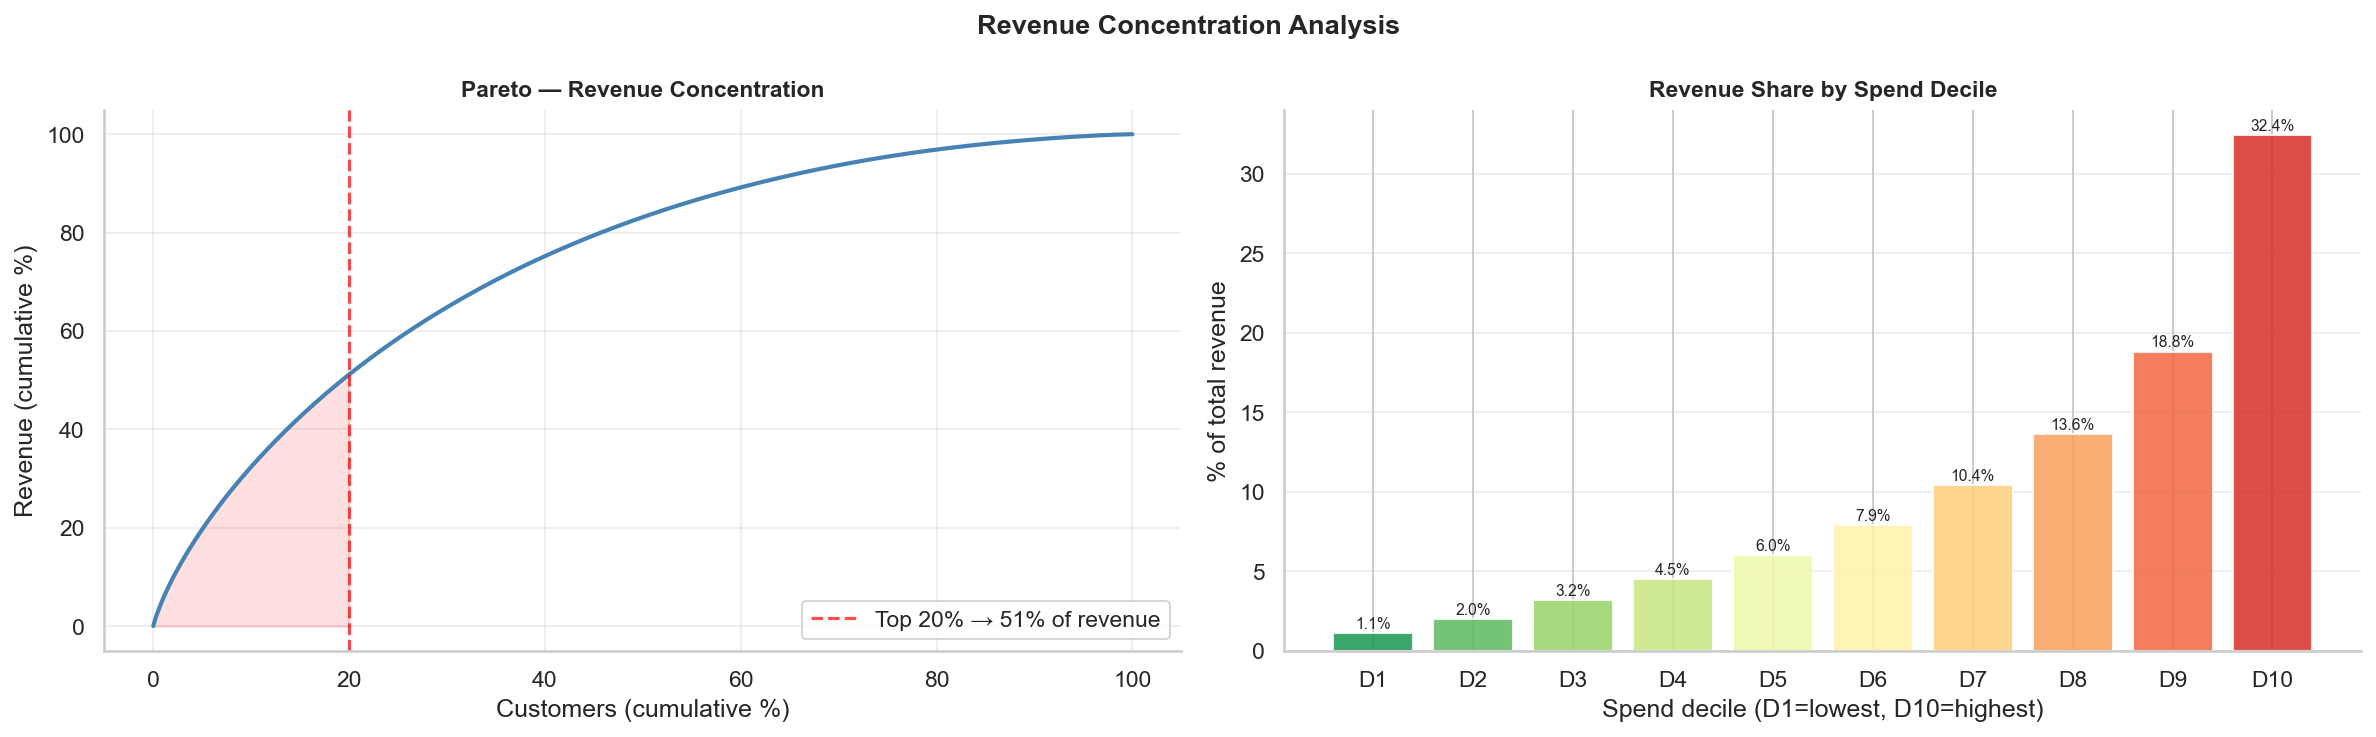
\includegraphics[width=\linewidth]{assets/eda_pareto.png}\\
    {\footnotesize Top 20\% of customers $\approx$ 71\% of revenue}
  \end{column}
\end{columns}
\end{frame}

% =============================================================================
\section{Methodology}
% =============================================================================

\begin{frame}{Our Approach: CRISP-DM End-to-End Pipeline}
\centering
\begin{columns}[c]
  \begin{column}{0.18\textwidth}\centering
    \textbf{Data}\\{\small 4 sources\\102K rows\\24 months}
  \end{column}
  \begin{column}{0.02\textwidth}\centering$\rightarrow$\end{column}
  \begin{column}{0.18\textwidth}\centering
    \textbf{Features}\\{\small 24 variables\\RFM + behaviour\\+ email}
  \end{column}
  \begin{column}{0.02\textwidth}\centering$\rightarrow$\end{column}
  \begin{column}{0.18\textwidth}\centering
    \textbf{UMAP}\\{\small 3D reduction\\n\_neighbors=30\\non-linear}
  \end{column}
  \begin{column}{0.02\textwidth}\centering$\rightarrow$\end{column}
  \begin{column}{0.18\textwidth}\centering
    \textbf{GMM K=6}\\{\small full covariance\\10 inits\\seed=42}
  \end{column}
  \begin{column}{0.02\textwidth}\centering$\rightarrow$\end{column}
  \begin{column}{0.18\textwidth}\centering
    \textbf{Strategy}\\{\small CLV model\\ROI scenarios\\roadmap}
  \end{column}
\end{columns}

\vspace{1.0em}
\begin{columns}[c]
  \begin{column}{0.3\textwidth}
    \begin{block}{Why UMAP?}
    \small Preserves non-linear local structure in behavioural data;
    better cluster separation than PCA on this manifold.
    \end{block}
  \end{column}
  \begin{column}{0.3\textwidth}
    \begin{block}{Why GMM?}
    \small Soft probabilistic assignments; handles elliptical, overlapping
    clusters; posterior probability = assignment confidence.
    \end{block}
  \end{column}
  \begin{column}{0.3\textwidth}
    \begin{block}{Why K=6?}
    \small Three convergent criteria: Silhouette peak, BIC inflection,
    posterior stability at 96.5\% $>$0.80. Details on next slide.
    \end{block}
  \end{column}
\end{columns}
\end{frame}

% =============================================================================
\section{Segments}
% =============================================================================

\begin{frame}{Six Behaviourally Distinct Segments}
\centering
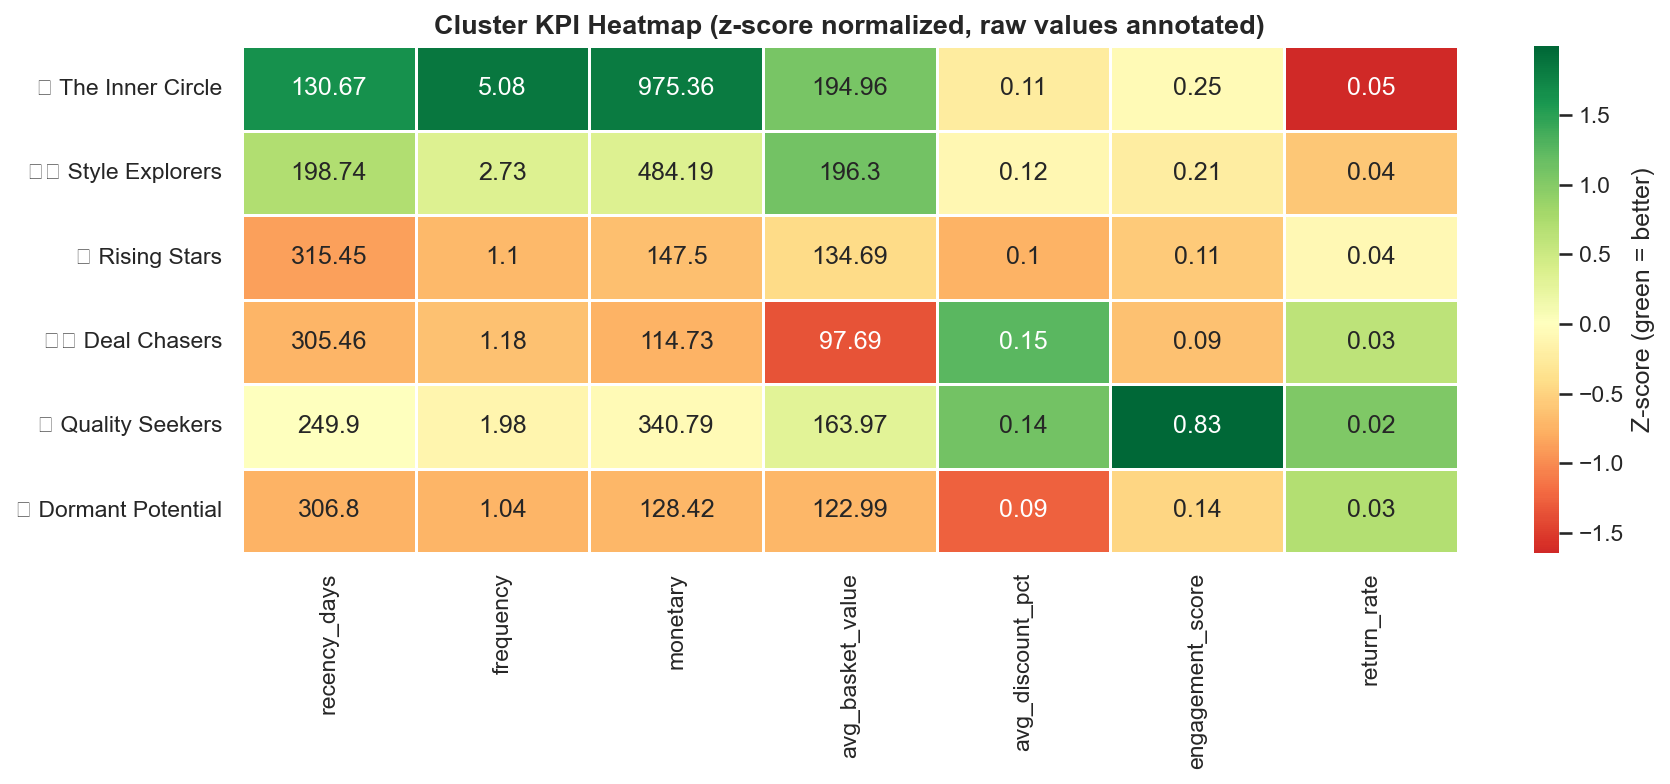
\includegraphics[width=0.62\textwidth]{assets/cluster_heatmap.png}
\hfill
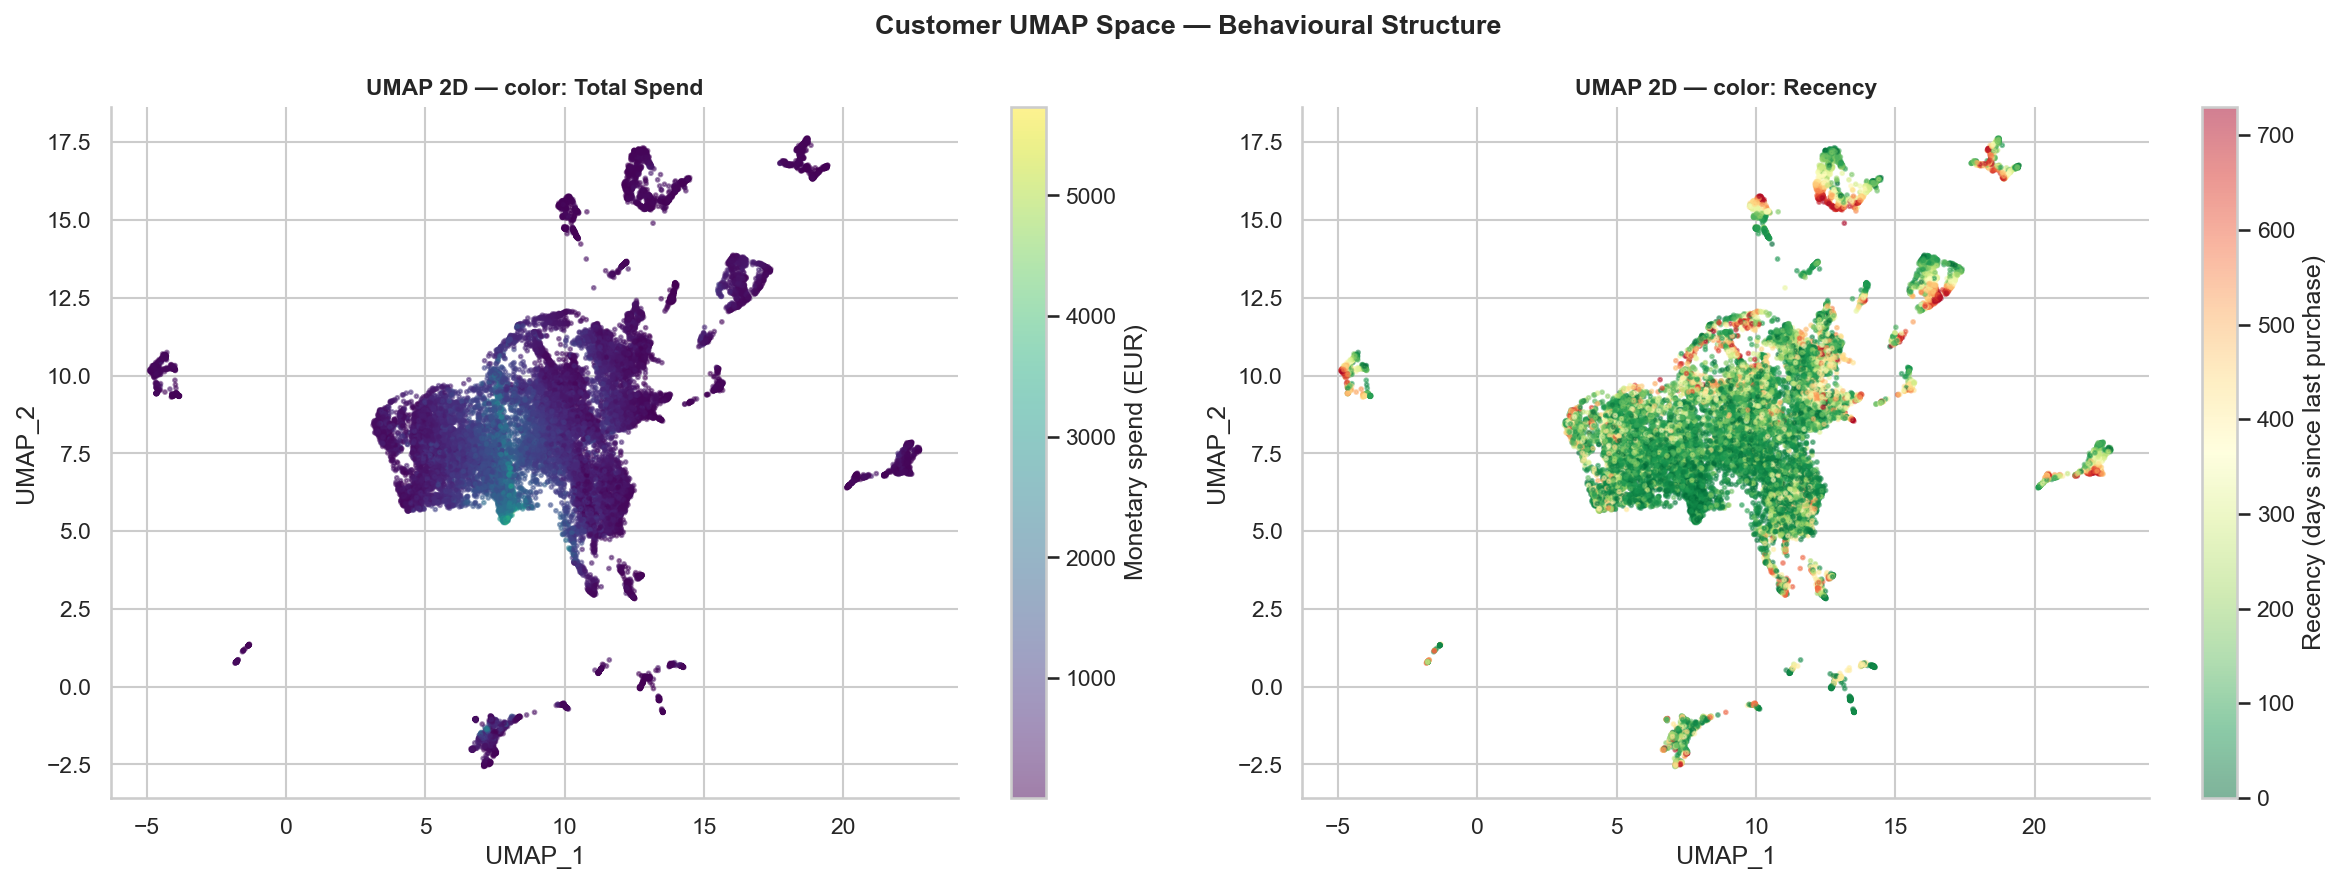
\includegraphics[width=0.35\textwidth]{assets/umap_space.png}
\vspace{0.3em}\\
{\footnotesize
  Silhouette 0.419 $\cdot$ Davies--Bouldin 0.760 $\cdot$
  Calinski--Harabasz 10{,}975 $\cdot$ GMM confidence (avg) 0.983}
\end{frame}

\begin{frame}{The Value Segments: Inner Circle \& Aspirational}
\begin{columns}[T]
  \begin{column}{0.48\textwidth}
    \textbf{\color{accent}Inner Circle} --- \textit{Loyal VIPs}
    \begin{itemize}\small
      \item Highest spend and frequency
      \item Strong email engagement (2.4$\times$ avg open rate)
      \item At-risk from competitor acquisition
    \end{itemize}
    \textbf{Strategy:} loyalty tier + early access + event invites.\\
    Investment: \euro55K $\rightarrow$ Uplift: \euro321K (5.1$\times$).
  \end{column}
  \begin{column}{0.48\textwidth}
    \textbf{\color{accent}Aspirational} --- \textit{Infrequent Premium Buyers}
    \begin{itemize}\small
      \item High avg basket, low visit frequency
      \item Occasion-driven purchases
      \item Highest unactivated CLV potential
    \end{itemize}
    \textbf{Strategy:} personalised reactivation + curated new arrivals.\\
    Investment: \euro20K $\rightarrow$ Uplift: \euro11K (0.6$\times$).
  \end{column}
\end{columns}
\vspace{0.5em}
\centering
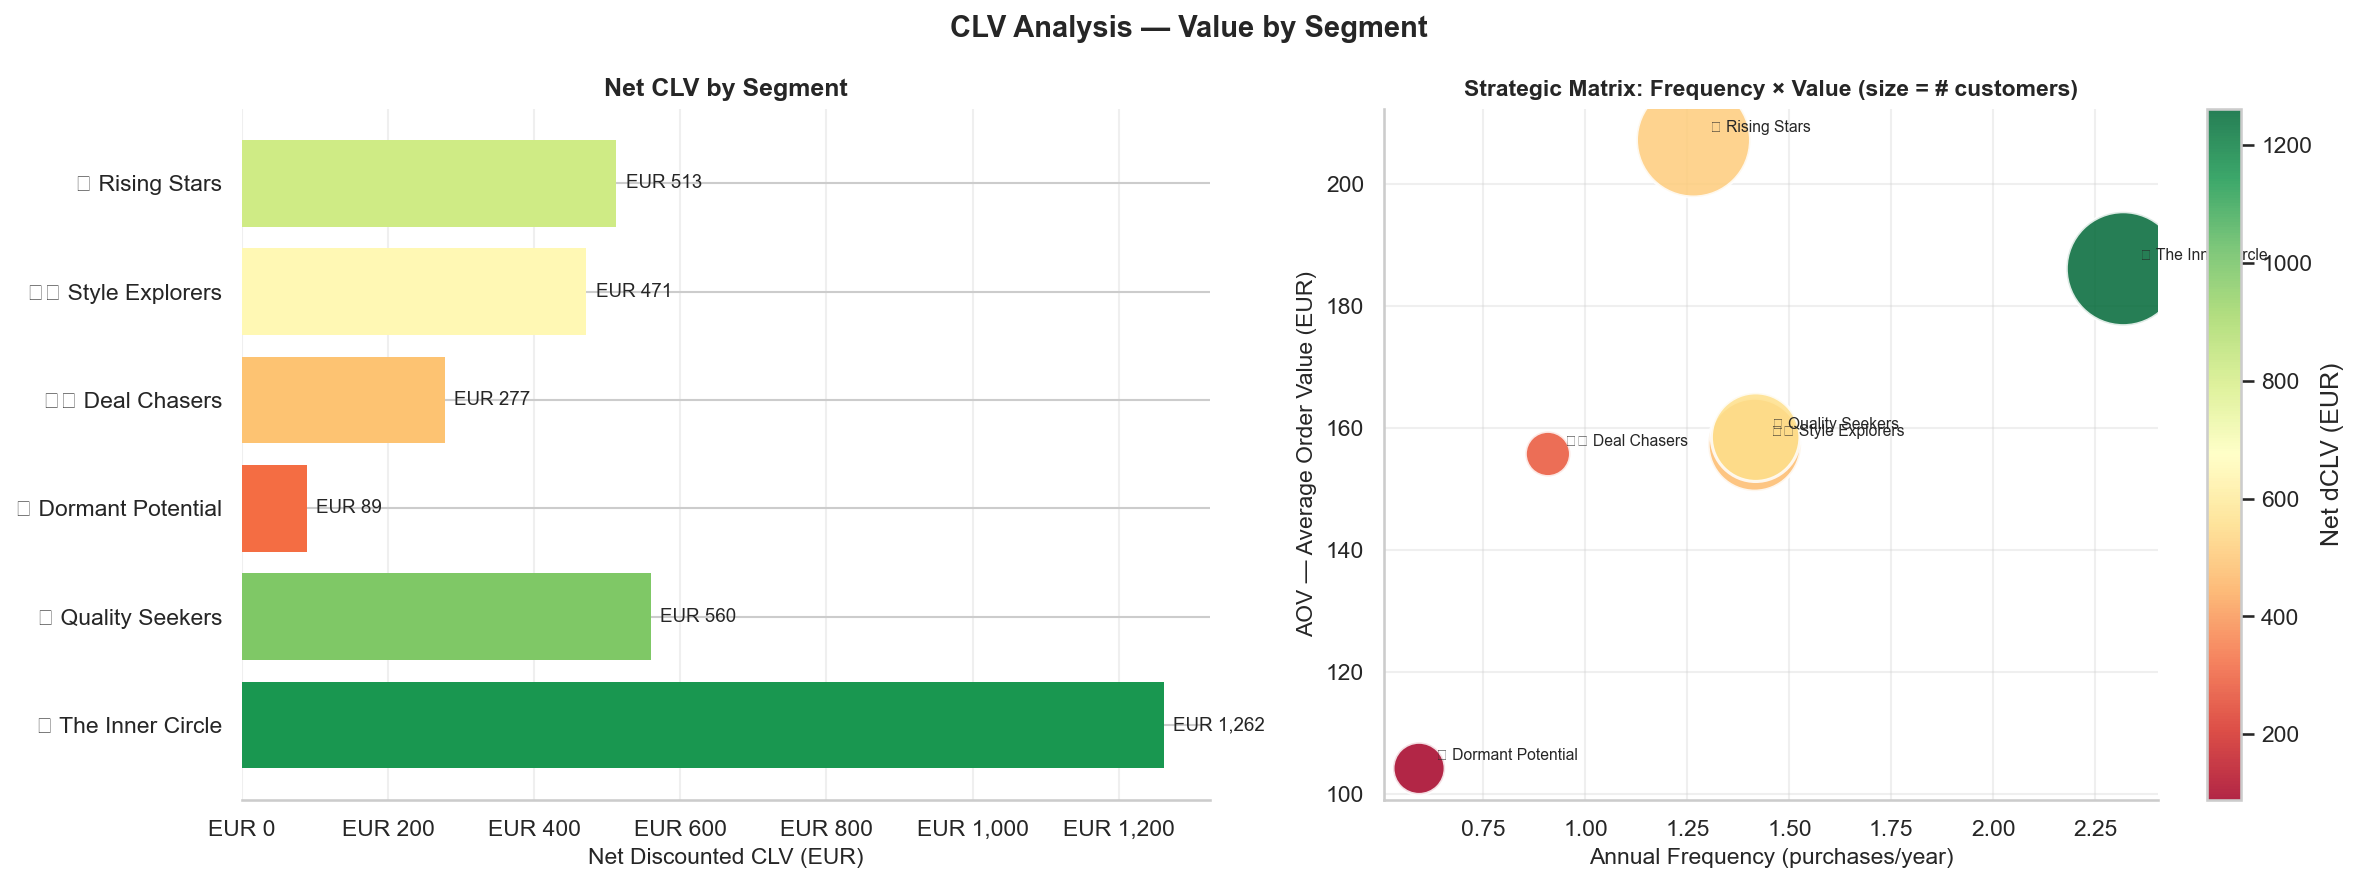
\includegraphics[width=0.55\textwidth]{assets/clv_analysis.png}
\end{frame}

\begin{frame}{The Challenge Segments: Deal Chasers \& Quality Seekers}
\begin{columns}[T]
  \begin{column}{0.48\textwidth}
    \textbf{\color{accent}Deal Chasers} --- \textit{Promotion-Driven}
    \begin{itemize}\small
      \item High frequency, low net margin
      \item Purchase only during discount windows
      \item Full-price conversion rate near zero
    \end{itemize}
    \textbf{Strategy:} A/B test bundle offers vs.\ discount;\\
    shift 20\% to full-price behaviour.\\
    Investment: \euro20K $\rightarrow$ Uplift: \euro4K (0.2$\times$).
  \end{column}
  \begin{column}{0.48\textwidth}
    \textbf{\color{accent}Quality Seekers} --- \textit{High-Return Customers}
    \begin{itemize}\small
      \item Above-average return rate (size/fit friction)
      \item Moderate spend; loyal if fit solved
    \end{itemize}
    \textbf{Strategy:} ML Size Advisor deployment;\\
    target $-$8\,pp return rate reduction.\\
    Investment: \euro15K $\rightarrow$ Uplift: \euro1K (0.1$\times$).\\[4pt]
    \small\textit{Note: low direct ROI; strategic value is margin\\
    recovery and NPS improvement.}
  \end{column}
\end{columns}
\end{frame}

% =============================================================================
\section{Financial Case}
% =============================================================================

\begin{frame}{Portfolio CLV: \euro16.2M Long-Run Value}
\begin{columns}[T]
  \begin{column}{0.52\textwidth}
    \centering
    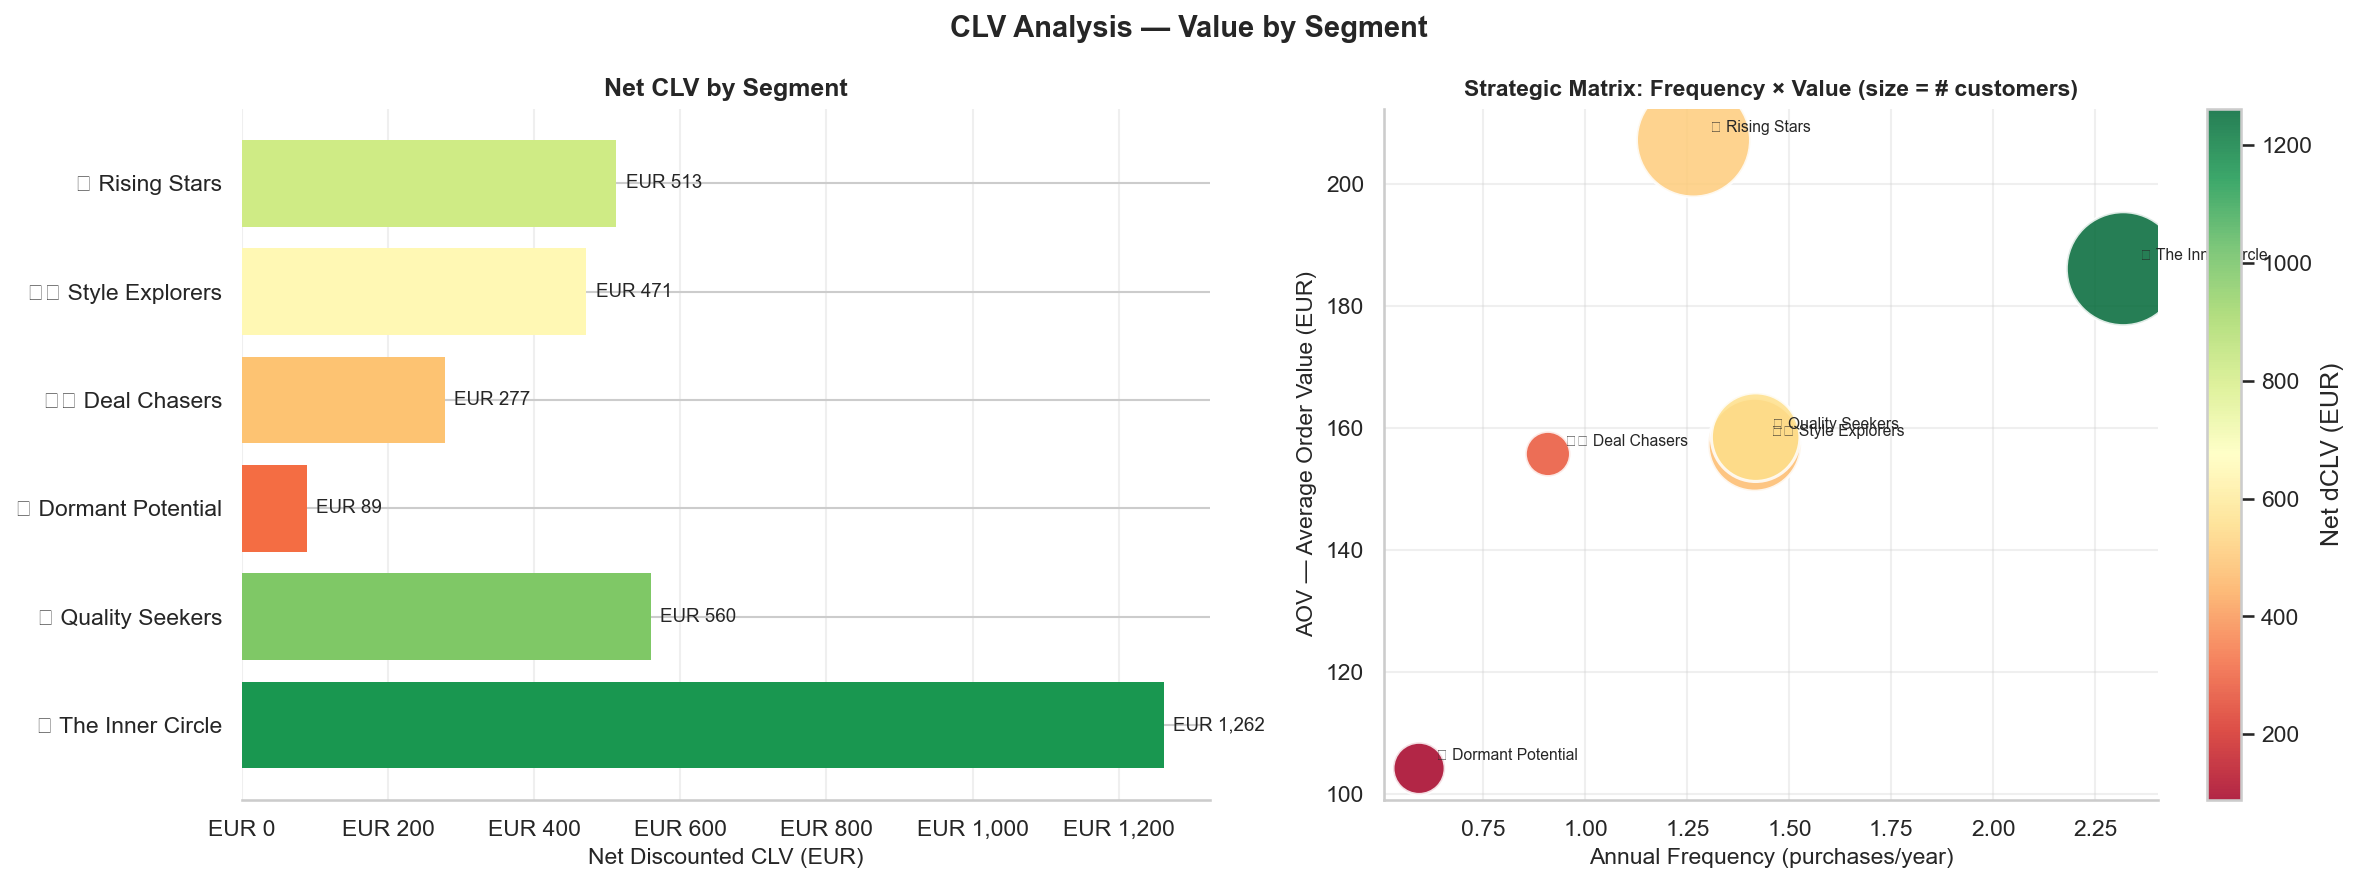
\includegraphics[width=\linewidth]{assets/clv_analysis.png}
  \end{column}
  \begin{column}{0.45\textwidth}
    \textbf{Discounted CLV model}\\
    {\small $\text{dCLV}_i = \frac{r_i \cdot m_i}{1+d - r_i}$ \quad
    WACC proxy $d=10\%$}

    \vspace{0.5em}
    \begin{tabular}{@{}lr@{}}
    \toprule
    \textbf{Segment} & \textbf{dCLV share} \\
    \midrule
    Inner Circle      & $\sim$XX\% \\
    Aspirational      & $\sim$XX\% \\
    Deal Chasers      & $\sim$XX\% \\
    Dormant Potential & $\sim$XX\% \\
    Style Explorers   & $\sim$XX\% \\
    Quality Seekers   & $\sim$XX\% \\
    \midrule
    \textbf{Total}    & \textbf{\euro16{,}187{,}953} \\
    \bottomrule
    \end{tabular}
    \vspace{0.3em}\\
    {\footnotesize Managerial reference; not a financial forecast.}
  \end{column}
\end{columns}
\end{frame}

\begin{frame}{ROI Framework: \euro140K Investment $\rightarrow$ \euro342K Uplift}
\centering
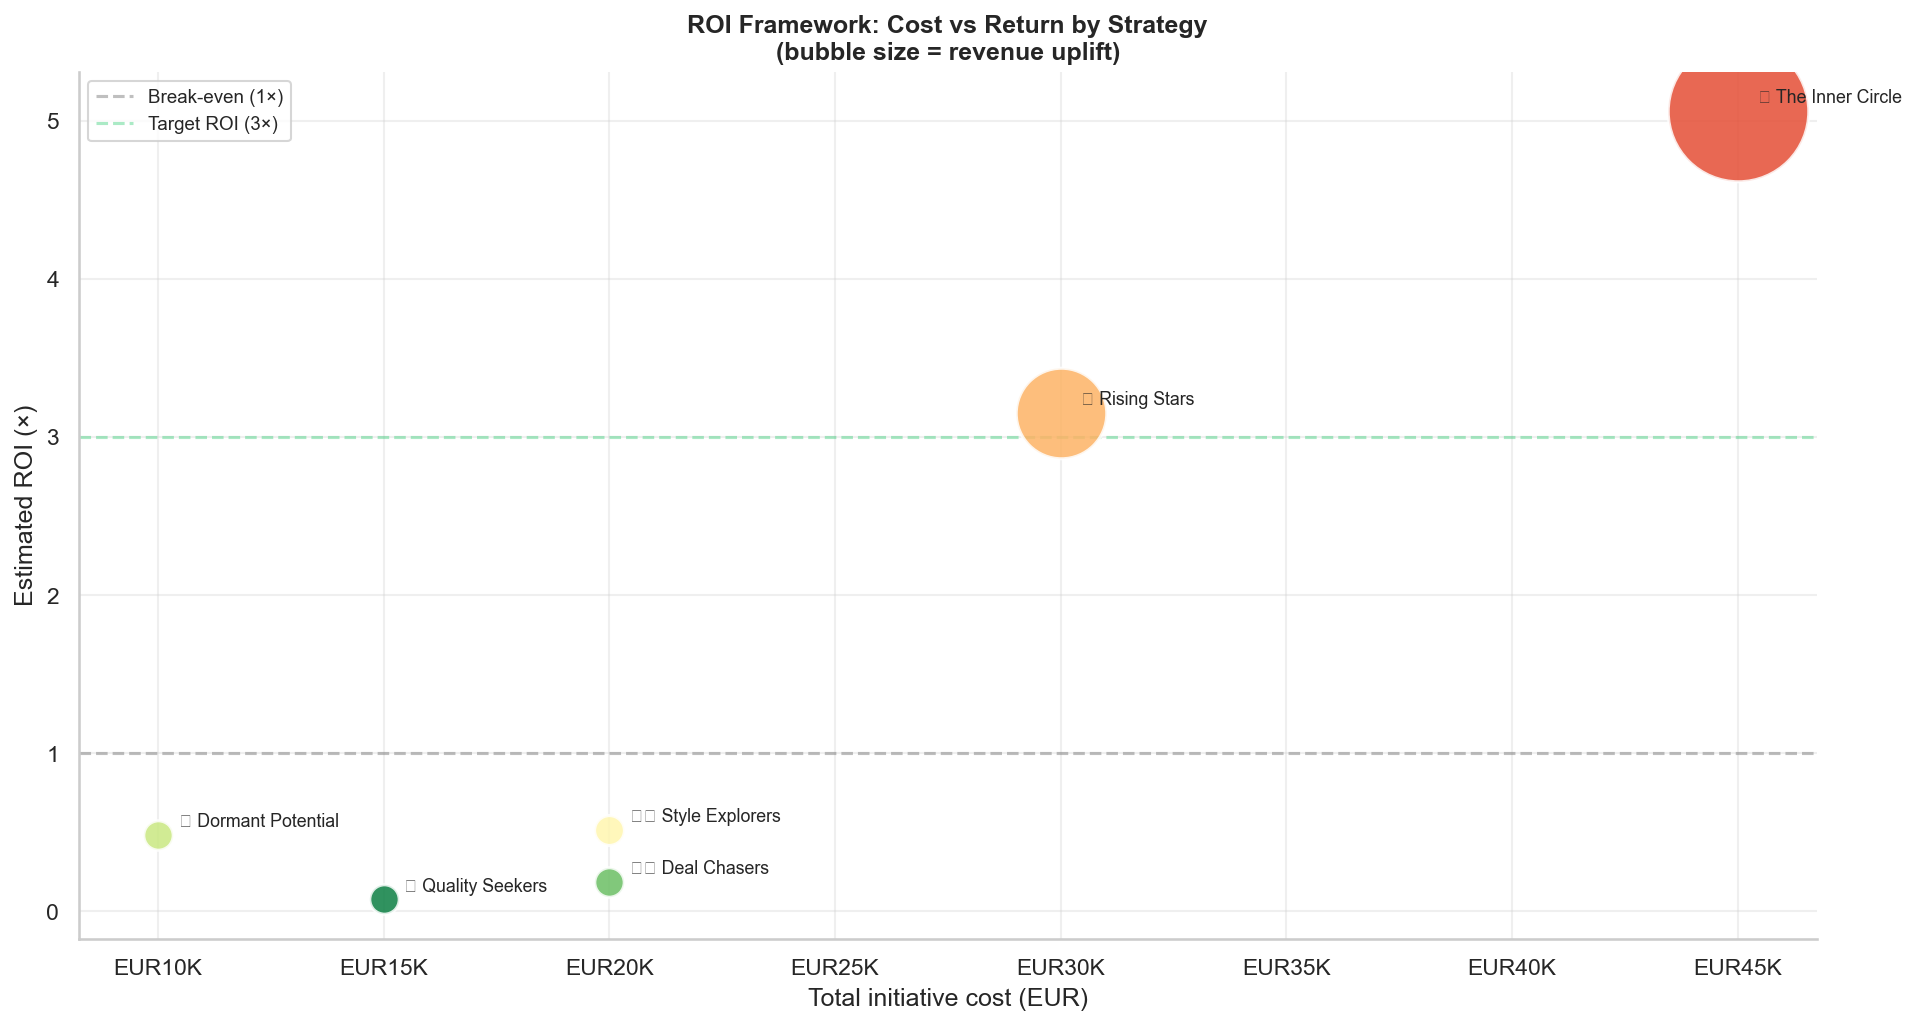
\includegraphics[width=0.70\textwidth]{assets/roi_framework.png}

\vspace{0.3em}
\begin{columns}[c]
  \begin{column}{0.22\textwidth}\centering
    \textbf{\euro140K}\\{\small annual investment}
  \end{column}
  \begin{column}{0.22\textwidth}\centering
    \textbf{\euro342K}\\{\small projected uplift}
  \end{column}
  \begin{column}{0.22\textwidth}\centering
    \textbf{2.4$\times$}\\{\small portfolio multiple}
  \end{column}
  \begin{column}{0.30\textwidth}\centering
    \textbf{5.1$\times$}\\{\small Inner Circle alone}
  \end{column}
\end{columns}
{\footnotesize\textit{Scenario estimates; all assumptions benchmarked to published literature.
  Require A/B validation before budgeting.}}
\end{frame}

% =============================================================================
\section{Roadmap}
% =============================================================================

\begin{frame}{Implementation Roadmap}
\begin{columns}[T]
  \begin{column}{0.32\textwidth}
    \textbf{Phase 1 --- Months 1--3}
    \begin{itemize}\small
      \item Deploy Inner Circle loyalty programme
      \item Set up weekly segmentation monitoring dashboard
      \item Establish A/B test framework for Inner Circle
    \end{itemize}
  \end{column}
  \begin{column}{0.32\textwidth}
    \textbf{Phase 2 --- Months 3--6}
    \begin{itemize}\small
      \item Launch Aspirational reactivation campaign
      \item A/B test Deal Chaser bundle vs.\ discount offers
      \item Pilot ML Size Advisor for Quality Seekers
    \end{itemize}
  \end{column}
  \begin{column}{0.32\textwidth}
    \textbf{Phase 3 --- Month 6+}
    \begin{itemize}\small
      \item Read A/B results; update CLV model with retention lift
      \item Retrigger segmentation if Silhouette drops below 0.34
      \item Expand to Dormant Potential win-back\\
            (3-touch sequence)
    \end{itemize}
  \end{column}
\end{columns}
\vspace{0.6em}
\begin{block}{Monitoring Trigger}
\small Refresh segmentation if: (a) segment size distribution drifts $>$10\%,
(b) Silhouette drops below 0.34, or (c) retailer adds a new product category.
\end{block}
\end{frame}

% =============================================================================
\section{Conclusions}
% =============================================================================

\begin{frame}{Conclusions \& Limitations}
\begin{columns}[T]
  \begin{column}{0.52\textwidth}
    \textbf{What we found}
    \begin{itemize}
      \item 6 behaviourally distinct, interpretable segments confirmed
        by three independent validation criteria
      \item Inner Circle (top segment) alone justifies the \euro140K
        investment at 5.1$\times$ return
      \item Uniform marketing is provably suboptimal: Deal Chasers and
        Quality Seekers require opposite strategies
      \item Portfolio dCLV of \euro16.2M gives an investment sizing anchor
    \end{itemize}
  \end{column}
  \begin{column}{0.45\textwidth}
    \textbf{Honest limitations}
    \begin{itemize}
      \item dCLV is a lower bound: right-censored window
        under-estimates recently acquired customers
      \item ROI figures are scenario estimates, not forecasts;
        all behavioural assumptions require A/B validation
      \item No holdout set: internal validation only
      \item Operational constraint (6 campaigns/cycle) used as
        secondary tie-breaker, not primary K criterion
    \end{itemize}
  \end{column}
\end{columns}
\vspace{0.5em}
\centering
{\large\color{accent}\textbf{The data says: stop averaging, start differentiating.}}
\end{frame}

% --- Thank you ----------------------------------------------------------------
\begin{frame}[plain]
\centering\vspace{1.5cm}
{\LARGE\color{navy}\textbf{Thank you}}\\[0.6em]
{\large\color{navy!70} Questions \& Discussion}\\[1.4em]
{\small
  \begin{tabular}{ll}
    $\langle$NOME 1$\rangle$ & $\langle$email 1$\rangle$ \\
    $\langle$NOME 2$\rangle$ & $\langle$email 2$\rangle$ \\
    $\langle$NOME 3$\rangle$ & $\langle$email 3$\rangle$ \\
    $\langle$NOME 4$\rangle$ & $\langle$email 4$\rangle$ \\
  \end{tabular}
}\\[1.2em]
{\footnotesize Fully reproducible via \texttt{master\_segmentation.ipynb} $\cdot$
  technical\_report.pdf available on request}
\end{frame}

\end{document}
